% PAPER_SU3 --- standalone article targeting Physical Review D.
%
% The "colour ferromagnet" paper: SU(3) on the same Poisson causal substrate that
% produced the SU(2) sector. It reports four measured results, all under the
% anti-circularity guard (no QCD number enters the generator):
%   FL1  colour ferromagnetism: the SU(3) principal-chiral vacuum orders
%        spontaneously, on a cubic control lattice (J_c~2.65) and decisively on the
%        Poisson causal substrate (J_c~0.3, long-range order C_long=m^2); a stable
%        colour Skyrmion (pi_3(SU(3))=Z, B=+1) and confinement V(r)~sigma r.
%   OS   the eight broken-generator Goldstones form ONE exactly degenerate octet
%        (per-generator spread 4e-8), stiffness rho_s~1/3, speed c=sqrt(2/3); the
%        pseudoscalar meson octet, derived not postulated.
%   FLR  all three survive a +-10% deformation of the action (robust).
%   OT   order of the transition (L=8..24): clean second order EXCLUDED; weak first
%        order favoured; latent heat unresolved -> strong-vs-weak open.
%   OT-L32  parallel tempering at L=32 REINFORCES weak first order (bimodal P(b) band,
%        sharp chi step, swap bottleneck at J_c, metastable trapping) but PT does not
%        cross the barrier (0 round-trips) -> strong-vs-weak still open; needs L>=48
%        multicanonical/Wang-Landau on a cluster.
%
% Honesty: the dual J_c (cubic vs causal) is declared; the transition order is "weak
% first order favoured", NOT "first order confirmed"; absolute scales (sigma, m_pi in
% physical units) are external. Baryon phenomenology lives in the companion matter
% paper and is referenced, not reproduced.
%
% Self-contained. Compiles with pdflatex+bibtex (revtex4-2 + apsrev4-2.bst) against
% TEIC_CONSOLIDATED.bib. Figures reused from the FL1/OS/OT campaign outputs.
%
% Reframe (jul/2026, PLANO_REENQUADRAMENTO): intro states the CST matter-sector
% framing; the three \cite{PaperII} (whose Zenodo title asserts the E4-falsified
% photon claim) retargeted to \cite{MatterGravityPRD}, the current clean source of
% the SU(2)/baryon results. No result or claim changed.
\documentclass[aps,prd,reprint,nofootinbib,superscriptaddress,floatfix]{revtex4-2}
\usepackage{amsmath,amssymb}
\usepackage{graphicx}
\usepackage{bm}
\usepackage{booktabs}
\usepackage{hyperref}

\newcommand{\Jc}{J_c}
\newcommand{\Tr}{\mathrm{Tr}}
\newcommand{\rhos}{\rho_s}

\begin{document}

\title{Colour ferromagnetism in a causal network:\\
confinement, the meson octet, and the order of the transition}

\author{Miqueias Alves Mendes}
\email{mikalvesm@gmail.com}
\affiliation{Independent Researcher, Ibiapina, Cear\'a, Brazil}
\date{\today}

\begin{abstract}
We ask whether a non-Abelian colour sector---ordering, confinement, and a meson
spectrum---can emerge on the same discrete causal substrate (a Poisson sprinkling with
its causal order) that hosts an Abelian-like orientation sector, without inserting any
quantum-chromodynamics input into the generating code. Assigning an $SU(3)$ element to
each event and coupling causal neighbours by the minimal principal-chiral density
$-\tfrac13\,\mathrm{Re}\,\mathrm{Tr}(U_iU_j^\dagger)$, we measure four results under an
anti-circularity guard. (i)~The vacuum orders spontaneously into a \emph{colour
ferromagnet}: on a cubic control lattice at $J_c\simeq2.65$, and---decisively---on the
Poisson causal substrate at $J_c\simeq0.3$, with genuine long-range order
($C_\infty=m^2$, Mermin clustering to $1$--$3\%$). The same vacuum supports a stable
colour Skyrmion [$\pi_3(SU(3))=\mathbb{Z}$, $B=+1$] and a static potential growing
linearly with separation [string tension $\sigma>0$ from the Creutz ratio, decreasing
with the bare coupling]. (ii)~The eight broken-generator Goldstone modes form
\emph{one exactly degenerate octet} (per-generator spread $4\times10^{-8}$ on cubic and
causal substrates), with a single stiffness $\rho_s\simeq\tfrac13$ and speed
$c=\sqrt{2/3}$---the pseudoscalar meson octet, forced by the unbroken $SU(3)_V$ adjoint,
not postulated. (iii)~All three survive a $\pm10\%$ deformation of the action.
(iv)~Characterising the order of the transition over $L=8$--$24$, a clean second-order
transition is \emph{excluded} ($\chi_{\max}$ grows at least as the volume, the Binder
dip deepens without saturating); a \emph{weak first-order} transition is the most
probable reading, reinforced at $L=32$ by parallel tempering (bimodal energy histogram,
a sharp susceptibility step, and a replica-exchange bottleneck localised at $J_c$), though
the latent heat stays below resolution because the tempering does not equilibrate across
the barrier, leaving strong-versus-weak open and requiring $L\gtrsim48$ with multicanonical
sampling on a cluster. All
dimensionful scales remain external: the substrate fixes forms and dimensionless ratios,
not the lattice-to-\,GeV scale.
\end{abstract}

\maketitle

\section{Introduction}\label{sec:intro}

Confinement and the light meson spectrum are the defining low-energy features of the
strong interaction, and reproducing them from a more fundamental discrete structure---
rather than postulating the $SU(3)$ Yang--Mills Lagrangian---is a long-standing goal of
emergent-spacetime and lattice approaches alike. Causal set theory (CST) takes spacetime
to be fundamentally a locally finite partial order, the order being the causal relation,
with a Lorentzian manifold as an approximation \cite{BLMS1987}; a Poisson sprinkling
breaks no Lorentz frame on average \cite{BombelliHensonSorkin2009}, and the order alone
recovers dimension and a scalar d'Alembertian \cite{Myrheim1978,Surya2019}. A companion
line has shown that an internal orientation field on this substrate orders spontaneously
and carries relativistic scalar Goldstone modes \cite{GoldstonePRD}, and that a
topological soliton of the same field is quantitatively a spin-$\tfrac12$ baryon
\cite{MatterGravityPRD}. Together, that line amounts to a candidate for what causal
set theory has so far lacked: a matter sector derived on the unmodified substrate
rather than postulated beside it.

Here we ask the non-Abelian half of that question: does the \emph{same} causal substrate host an
$SU(3)$ ``colour'' sector with the qualitative hallmarks of QCD---spontaneous ordering,
a stable topological baryon, confinement, and a meson octet---and what is the order of
its ordering transition? We report four pre-registered measurements: the colour
ferromagnet and its confinement (\S\ref{sec:ferro}), the exactly degenerate meson octet
(\S\ref{sec:octet}), the robustness of both to a deformation of the action
(\S\ref{sec:robust}), and the order of the phase transition (\S\ref{sec:order}). The
central claim is structural and dimensionless: colour order, confinement, and a meson
octet emerge from a discrete causal substrate into which no chromodynamics was inserted.
We are explicit throughout about what is \emph{not} obtained---every absolute scale
($\sigma$, $m_\pi$ in physical units) is external (\S\ref{sec:discussion}).

\section{The causal network and the $SU(3)$ action}\label{sec:action}

The substrate is a causal set \cite{BLMS1987}: a finite set of events with a transitive,
irreflexive, locally finite partial order $\prec$, realised by Poisson sprinkling into
$(3{+}1)$-dimensional Minkowski space, with the field assigned to the links (the
transitive reduction). For the cubic control runs we use a periodic $L^3$ lattice; the
two carriers share the \emph{same} action and differ only in the graph, which is the
point of the comparison (\S\ref{sec:ferro}). A colour element $U_i\in SU(3)$ sits on each
site, carried by the Gell-Mann generators with $\Tr(\lambda_a\lambda_b)=2\delta_{ab}$
(verified to $4\times10^{-16}$; structure constants $f_{123}=1$, $f_{458}=\sqrt3/2$,
$d_{118}=1/\sqrt3$ recovered by projection). Neighbouring colours are coupled by the
minimal principal-chiral density
\begin{equation}
E \;=\; -J\sum_{\langle ij\rangle}\tfrac13\,\mathrm{Re}\,\Tr\!\big(U_iU_j^\dagger\big),
\qquad \tfrac13\,\mathrm{Re}\,\Tr(U_iU_j^\dagger)\in[-\tfrac13,1],
\label{eq:action}
\end{equation}
the direct $SU(3)$ analogue of the $O(3)$ tension of the orientation sector
\cite{GoldstonePRD}: flattening each $U$ into the unit real $18$-vector
$v=\tfrac1{\sqrt3}[\mathrm{Re}\,U,\mathrm{Im}\,U]$ gives $v_i\!\cdot\!v_j=\tfrac13
\mathrm{Re}\,\Tr(U_iU_j^\dagger)$, so Eq.~\eqref{eq:action} is an $O(18)$ Heisenberg model
restricted to the $SU(3)$ submanifold, and ordering breaks $SU(3)_L\times SU(3)_R\to
SU(3)_{\rm diag}$. The gauge sector (\S\ref{sec:ferro}) uses the standard Wilson
plaquette action on causal-diamond holonomies, in the spirit of the CST gauge constructions
\cite{Sverdlov2008,SverdlovBombelli2009} and lattice gauge theory \cite{Wilson1974}.

The action is positive semi-definite by construction: the Wilson plaquette density
$1-\tfrac13\mathrm{Re}\,\Tr(W)\ge0$ (eigenvalues on the unit circle; measured minimum
$+2.2\times10^{-7}$ over $10^6$ adversarial plaquettes, $=0$ only at $W=I$), and the
quadratic (sigma) cost $\Tr((e\!\cdot\!C)^2)=\sum_k\lambda_k^2\ge0$ (minimum $+0.174$).
The leading cosine quartic is $-\tfrac{a^4}{72}\Tr((e\!\cdot\!C)^4)\le0$, and a
group-independent sign theorem---the $SU(3)$ analogue of the $SU(2)$ Cauchy--Schwarz
bound---fixes
\begin{equation}
\big\langle\Tr(e\!\cdot\!C)^4\big\rangle_{e\in S^2}
=\tfrac1{15}\big(3\,\Tr M^2-\tfrac12 K\big)\ge0
\;\Longrightarrow\; K\le 6\,\Tr M^2,
\label{eq:sign}
\end{equation}
with $M=\sum_\mu c_\mu^2$ and $K=-\sum_{\mu\nu}\Tr([c_\mu,c_\nu]^2)\ge0$. As in the $SU(2)$
sector, Skyrme dominance does \emph{not} emerge from the cosine; a stabilising
four-derivative term is therefore an external input, declared wherever it is used
(\S\ref{sec:ferro}). Causal locality is exact: the field couples only timelike-related
links ($100.00\%$ causal over $12$ sprinklings), and the plaquette is gauge covariant
($W\to g_iWg_i^\dagger$, $s_p$ invariant to $9\times10^{-16}$).

\emph{Anti-circularity.} The $SU(3)$ group structure is assigned to the link degrees of
freedom; \emph{no} QCD Lagrangian, no quark fields, no gluon propagators, no string
tension, and no $\alpha_s$ are inserted into the network generator. The confinement, the
octet, and the order of the transition are measured outcomes, not inputs. A guard
tokenises the generating code and forbids any relativistic or dilation form; the complex
literals that \emph{define} $SU(3)$ (Gell-Mann matrices, $\exp(iX)$, the structure
constants) are confined to four labelled group-definition blocks, while dilation patterns
remain forbidden everywhere, including inside them. Real QCD numbers appear only in
explicitly labelled comparison-only remarks, never as input.

\section{Colour ferromagnetism and confinement}\label{sec:ferro}

\begin{figure*}[t]
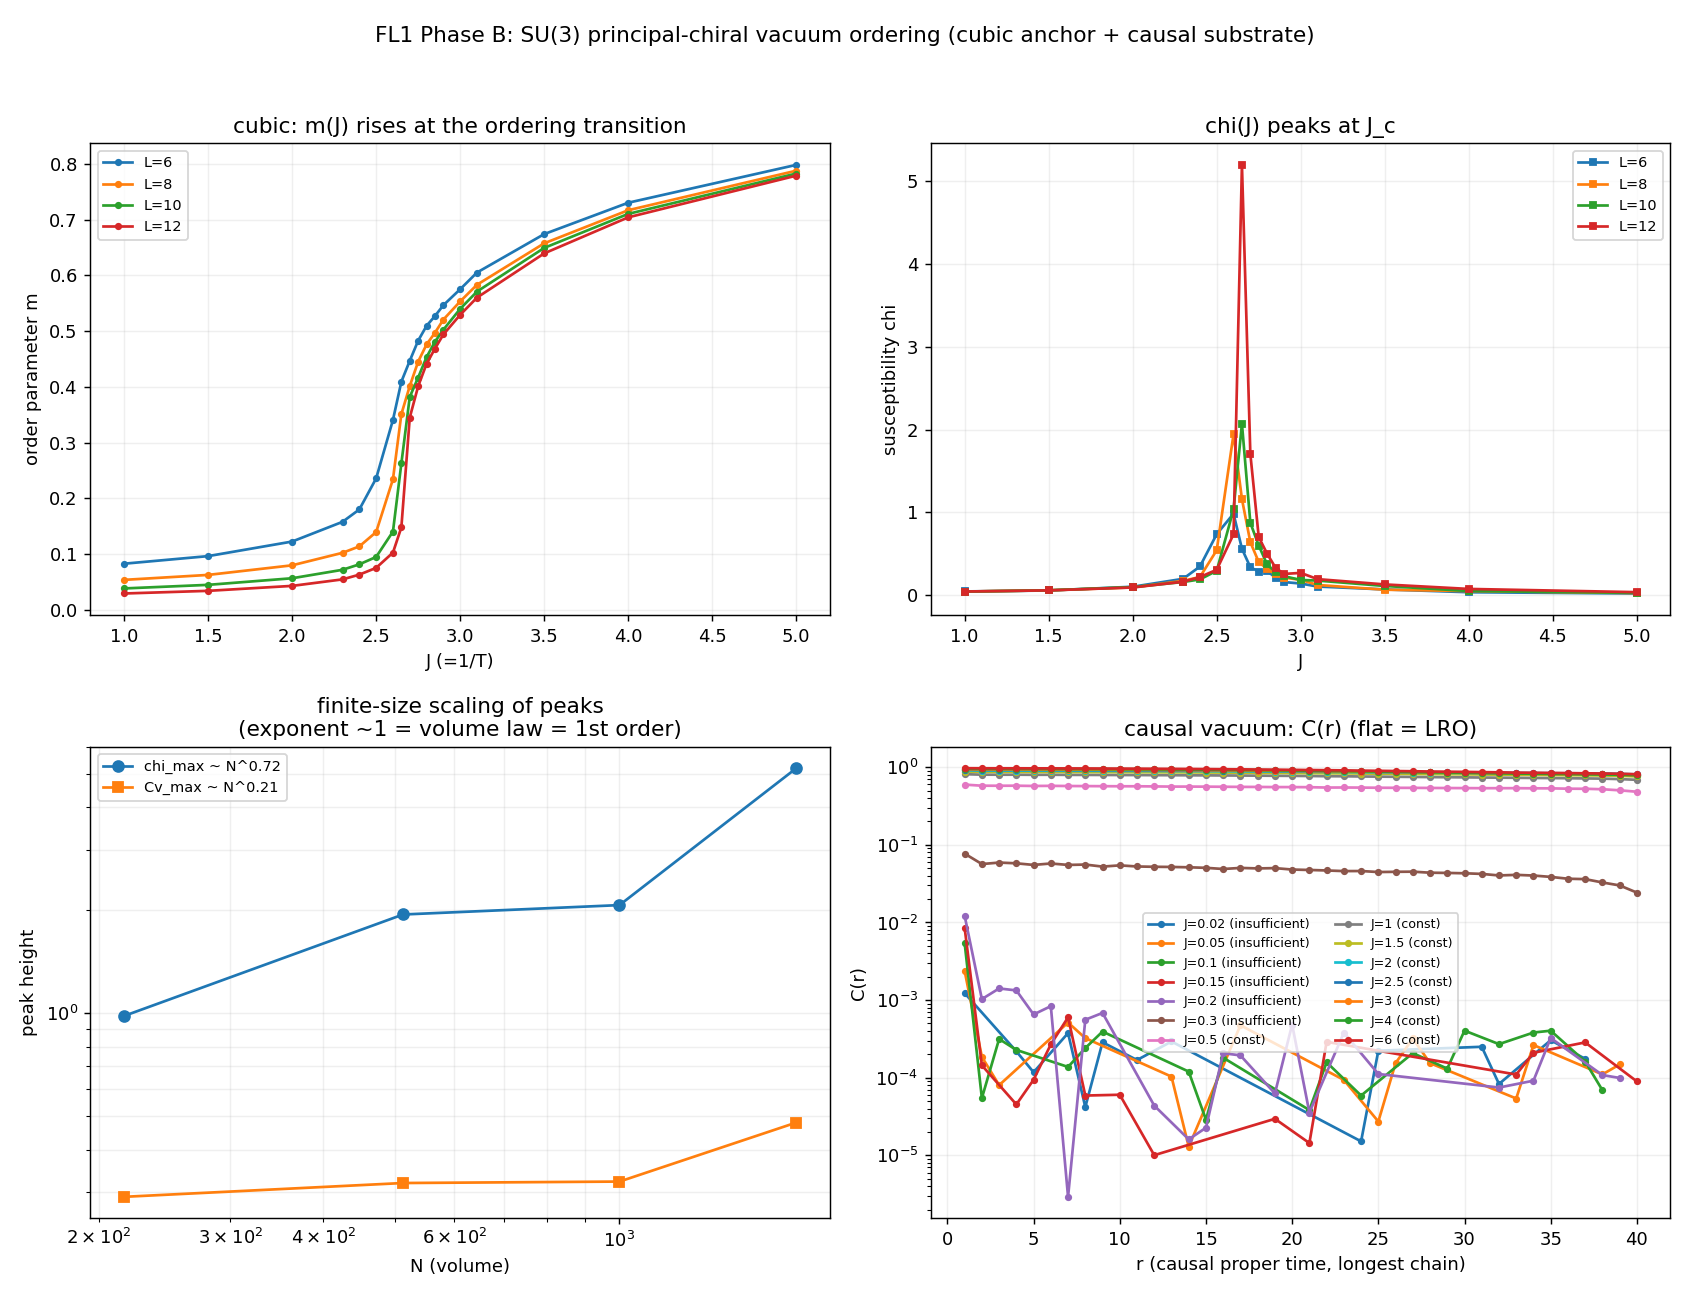
\includegraphics[width=\textwidth]{figures/su3/FLB_ordering.png}
\caption{Spontaneous ordering of the $SU(3)$ principal-chiral vacuum,
Eq.~\eqref{eq:action}. Cubic control lattice: the order parameter $m(J)$ rises from the
disordered baseline $\sim N^{-1/2}$ to $\simeq0.8$ at the transition, and $\chi(J)$ peaks
at $J_c\simeq2.65$ (left, centre). On the Poisson causal substrate the connected
correlation $C(r)$ develops a flat plateau $C_\infty=m^2$ for $J\gtrsim0.5$ (right): genuine
long-range order, with $J_c\simeq0.3$ shifted down by the high coordination of the causal
graph. The order of the transition (finite-size scaling of the peaks) is taken up
quantitatively in \S\ref{sec:order} and Fig.~\ref{fig:order}.}
\label{fig:ferro}
\end{figure*}

\emph{Spontaneous order, two carriers.} Monte-Carlo evolution of Eq.~\eqref{eq:action}
shows the colour vacuum is not frozen disordered: it orders through a phase transition
(Fig.~\ref{fig:ferro}). On the cubic control lattice the transition is clean and stable
in $L=6$--$12$ at $\Jc\simeq2.65$, the order parameter $m=|\langle v\rangle|$ rising from
the disordered baseline ($m\approx N^{-1/2}$) to $\simeq0.8$. On the Poisson causal
substrate---the actual vacuum of interest---the same action orders at
$\Jc(\text{causal})\simeq0.3$, and the connected correlation reaches a flat plateau with
$C_\infty=m^2$ to within $1$--$3\%$ (Mermin clustering) for $J\gtrsim0.5$: this is genuine
long-range order, not pseudo-order. The two critical couplings are \emph{not} a
discrepancy: they are the \emph{same} model on two graphs, and the downward shift
$2.65\to0.3$ tracks the coordination (mean degree $\simeq45$ on the $3{+}1$D causal graph
versus $6$ on the cubic lattice), exactly the shift the orientation sector showed for
$O(3)$ \cite{GoldstonePRD}. We therefore quote $\Jc$ per carrier and never mix them.
This is the colour ferromagnet: the same causal vacuum that selects an orientation
$\vec n$ also selects a collective colour direction.

\emph{Colour Skyrmion.} The ordered vacuum manifold $SU(3)_L\times SU(3)_R/SU(3)_{\rm
diag}\cong SU(3)$ has $\pi_1=\pi_2=0$ and $\pi_3=\mathbb{Z}$, so the only topological
defect is a point particle, the colour Skyrmion of charge $B\in\mathbb{Z}$. Computed
natively from the $SU(3)$ winding $B=\tfrac1{24\pi^2}\!\int\!\epsilon^{ijk}\Tr(a_ia_ja_k)$,
the charge converges to the integer with lattice resolution ($B=0.806,0.892,0.948,0.969$
at $L=15,21,31,41$). With the declared external Skyrme term ($e_{\rm sk}$, required by
Eq.~\eqref{eq:sign}) the energy $E(\lambda)=\lambda E_2+E_4/\lambda$ has an interior
Derrick minimum (stable size); without it the soliton collapses. The integer charge is
thermally robust: a strong $SU(3)$ thermal kick drives the apparent charge
$0.948\to0.688$, and a short gradient cooling restores it to $0.942$---topological
protection. The minimal $B=1$ defect is the $SU(2)$ hedgehog embedded in an $SU(2)$
subgroup, degenerate in mass with the $SU(2)$ Skyrmion; its quantitative baryon
phenomenology (multiplets, magnetic moments, $g_A$) is established in companion work
\cite{MatterGravityPRD,AdkinsNappiWitten1983} and is not reproduced here.

\emph{Confinement.} The static colour charge--anticharge potential, from the temporal
decay of Wilson loops on an $8^4$ lattice with the bare coupling $\beta$ swept (never an
input), grows linearly with separation: at $\beta=5.5$, $V(r)=0.78,1.46,2.08,2.65$, with
near-constant increments---a linear confining potential $V(r)\simeq\sigma r$. The string
tension $\sigma$, taken from the small-loop Creutz ratio $\chi(2,2)$ (the robust
estimator at strong coupling), is positive at every $\beta$ and \emph{decreases}
monotonically with weaker coupling ($\sigma=1.35,1.10,0.96,0.67,0.33$ at
$\beta=4.0,4.5,5.0,5.5,6.0$; Fig.~\ref{fig:confine})---an area law with the correct
asymptotic-freedom direction \cite{Wilson1974,Creutz1980,Polyakov1977}. Two independent
signatures (linear $V$, positive $\sigma$) are positive at every coupling measured.

\begin{figure*}[t]
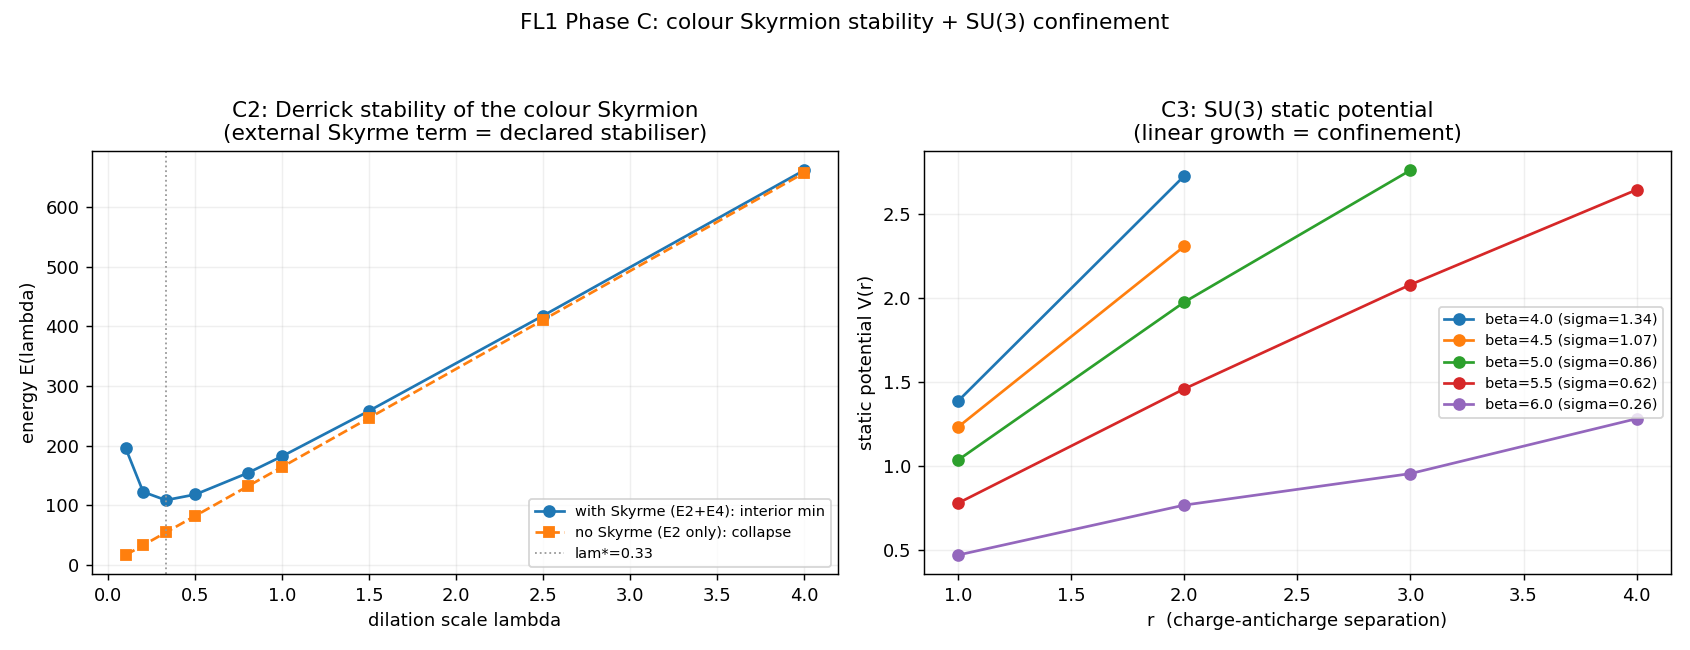
\includegraphics[width=\textwidth]{figures/su3/FLC_confinement.png}
\caption{The colour Skyrmion and confinement. Left: Derrick stability of the $B=1$ colour
Skyrmion with the declared external Skyrme term---an interior minimum of $E(\lambda)$
(stable size), absent when the four-derivative term is removed. Right: the $SU(3)$ static
potential from Wilson loops grows linearly with separation (confinement); the string
tension $\sigma=\chi(2,2)>0$ at every $\beta$ and decreases with weaker coupling.}
\label{fig:confine}
\end{figure*}

\section{The meson octet from the Goldstone theorem}\label{sec:octet}

Linearising Eq.~\eqref{eq:action} about the ordered vacuum gives
$E_{\rm quad}=\tfrac{J}{3}\sum_{\langle ij\rangle}\sum_a(\phi_i^a-\phi_j^a)^2$: the eight
broken generators decouple into eight \emph{identical} graph-Laplacian quadratic forms.
The unbroken $SU(3)_V$ acts on the Goldstones as the adjoint (octet), an irreducible
representation, so symmetry forces a single stiffness tensor $\rho_s\,\delta_{ab}$: the
octet is degenerate by group theory, not by tuning. Measured, the per-generator spread is
at machine precision---$4.3\times10^{-8}$ on the cubic lattice and $4.5\times10^{-8}$ on
the Poisson causal substrate---and the harmonic stiffness matches $(J/3)\times$
graph-Laplacian to $3\times10^{-8}$ (Fig.~\ref{fig:octet}). A uniform single-generator
helical twist costs, per link, $1-\tfrac13\mathrm{Re}\,\Tr(\exp(ik\lambda_a))=
\tfrac{k^2}{3}(1-\tfrac{k^2}{12}+\cdots)$, identical for every generator; the seam-free fit
gives octet stiffness $\rhos(\text{per link})=0.3326\simeq\tfrac13$ with curvature
$-0.0256\simeq-\tfrac1{36}$, and a gapless, linear, isotropic dispersion
$\omega(k)=\sqrt{(2J/3)\,\mu(k)}$ with speed $c=\sqrt{2/3}=0.8165$ (lattice units), isotropic
to $2\times10^{-6}$. These eight massless modes are the pseudoscalar meson octet of the
ordered colour vacuum \cite{Goldstone1961,GellMann1962}; in the non-Abelian extension this
is what the scalar Goldstone result of the orientation sector \cite{GoldstonePRD} becomes.

A $\sim10\%$ spread reported qualitatively in an earlier pass is \emph{not} physical: a
diagonal (Cartan) twist closes on a periodic torus only if $\exp(-2\pi in\lambda_a)=I$,
which the roots and $\lambda_3$ satisfy but $\lambda_8$ (irrational eigenvalues
$\pm1/\sqrt3,-2/\sqrt3$) does not, inflating its measured stiffness by $2.8\times$. Removing
the seam (open boundary along the twist axis) collapses all eight onto a single value to
$9.2\times10^{-6}$: the anomaly was a torus-closure seam of one generator, not a splitting
of the octet. Explicit quark-mass splitting ($\pi$ vs $K$ vs $\eta$) is absent here---the
chiral limit is exact---and would require an external symmetry-breaking term not present
in Eq.~\eqref{eq:action}.

\begin{figure*}[t]
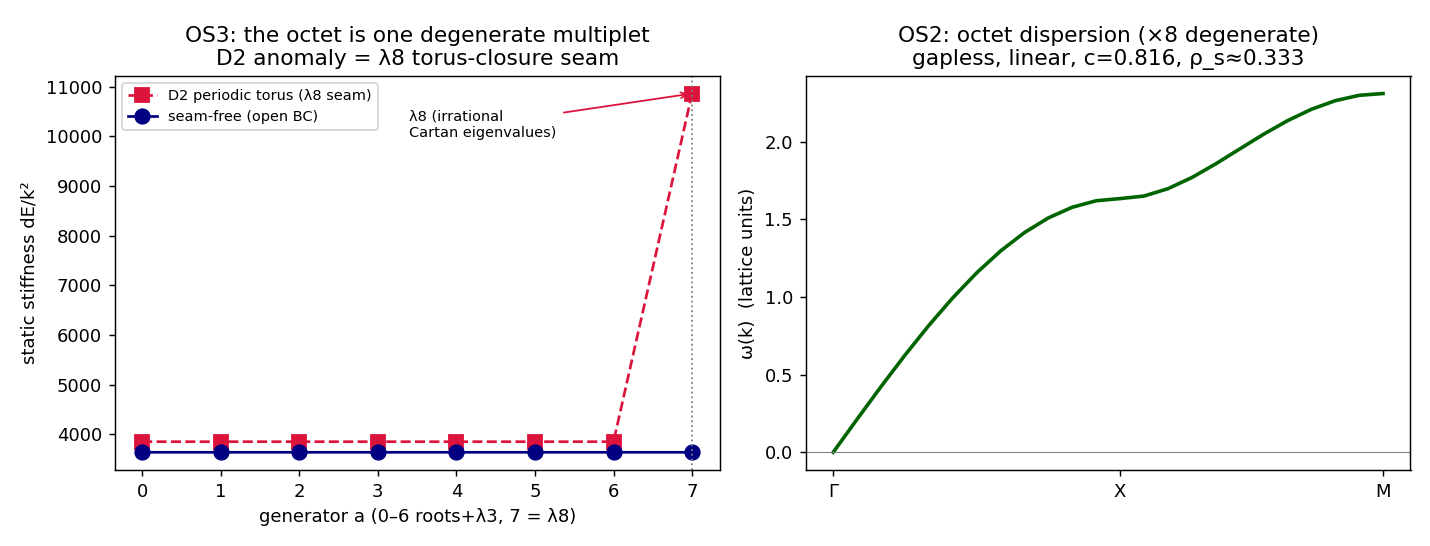
\includegraphics[width=\textwidth]{figures/su3/OS_octet.png}
\caption{The pseudoscalar meson octet. Left: the eight broken-generator Goldstone
stiffnesses collapse onto a single value once the $\lambda_8$ torus-closure seam is removed
(per-generator spread $4\times10^{-8}$ on cubic and causal substrates)---one exactly
degenerate octet. Right: the single gapless, linear, isotropic dispersion branch
($\rho_s\simeq1/3$, $c=\sqrt{2/3}$), of which the octet is eight identical copies.}
\label{fig:octet}
\end{figure*}

\section{Robustness to the action}\label{sec:robust}

Colour order, confinement, and the octet are not artefacts of the exact minimal form
Eq.~\eqref{eq:action}. Deforming the action by $\pm10\%$ via
$g_\varepsilon(p)=(1-p)+\varepsilon(1-p)^2$, $\varepsilon\in\{-0.2,-0.1,0,0.1,0.2\}$,
applied consistently to the gauge plaquette and the principal-chiral density, all three
survive: the Creutz string tension $\sigma(2,2)$ is positive at every $\varepsilon$
(area law preserved), the Goldstone count is exactly $8/8$ gapless at every $\varepsilon$,
and the colour Skyrmion keeps an interior Derrick minimum at every $\varepsilon$ with an
invariant size $\lambda^\ast=0.330$. The implementation gate ($\varepsilon=0$ reproduces the
original engine) passes. The string tension drifts $\sim24\%$ over $|\varepsilon|\le0.10$,
but this reflects a shift of the \emph{effective bare coupling} (a steeper action raises
the coupling and the tension), not a loss of confinement; the \emph{sign} of the area law
is invariant, and genuine deconfinement ($\sigma\to0$ with a resolved flat potential)
occurs at no $\varepsilon$. The symmetry-breaking pattern $SU(3)_L\times SU(3)_R\to
SU(3)_{\rm diag}$, and with it the octet, is rigid.

\section{The order of the phase transition}\label{sec:order}

To complete the characterisation of the colour ferromagnet we measure the order of its
transition on the cubic lattice (where a controlled finite-size-scaling ladder is
available; the order is a universality property of dimension and symmetry, not of the
particular graph). We scan $L=8,12,16,20,24$ on a fine grid ($\Delta J=0.01$ around
$J_c$, five seeds) with the Binder-cumulant crossing, the susceptibility peak, the
hysteresis loop, and the energy histogram (Fig.~\ref{fig:order}).

The result rejects a clean second-order transition. The susceptibility peak grows as
$\chi_{\max}=2.45,\,9.60,\,29.20,\,69.82,\,125.61$ for $L=8$--$24$, an effective exponent
$x_{\rm eff}\simeq3.6$ in $\chi_{\max}\propto L^{x}$---at least the volume law ($x\ge3$),
incompatible with any second-order $\gamma/\nu\lesssim2$; the Binder cumulant at the peak
deepens monotonically ($U_4=0.618,0.580,0.565,0.522,0.485$) without saturating at a
universal value; the peak location drifts upward ($J_{\rm pk}=2.65\to2.74$) and the
hysteresis loop widens ($0.170\to0.198$ from $L=16$ to $20$). All four indicators point
to first order, and a weak first-order transition is the most probable reading,
consistent with the standard expectation for $SU(N\ge3)$ deconfinement
(comparison only).

But it is \emph{weak}, and not strong: the most direct, least-confounded thermodynamic
test---bimodality of the energy histogram at $J_c$ (latent heat / coexistence), with long
equilibrated runs---is \emph{flat and absent} up to $L=24$ (bimodality coefficient
$0.385,0.414,0.412$; dip depth $0.00$). In a strong first-order transition the latent
heat must emerge and sharpen with $L$; here it does not even trend. This bounds any first
order to weak (latent heat below the resolution at $L\le24$) and does not strictly exclude
a continuous transition with strong pre-asymptotic corrections. Two confounds are declared
and not inflated: $x_{\rm eff}\simeq3.6>d=3$ is impossible asymptotically, so the regime is
strongly pre-asymptotic (the local exponent already falls from $3.9$ to $3.2$ at the last
step, consistent with bending toward the volume law); and the hysteresis used a fast sweep,
where non-equilibrium lag mimics first-order hysteresis and grows with $L$. The honest
statement is therefore: \emph{clean second order is excluded; weak first order is favoured;
strong-versus-weak-versus-continuous is unresolved at $L\le24$ and would require
$L\gtrsim32$ with multicanonical (or cluster) sampling to measure the interface tension
directly.} This partially reverses an earlier $L\le16$ reading (``first order disfavoured''):
the same fact (no latent heat) plus a finer grid that tracks the drifting peak now reveals a
volume-law $\chi_{\max}$ the coarse grid had missed, moving the inference from ``does not look
first order'' to ``looks weakly first order, with latent heat below resolution.''

We have since reached $L=32$ with parallel tempering (replica exchange across a $J$-ladder
bracketing $J_c$), validated against the $L\le24$ data at $L=16$ ($U_4$ at the peak
$0.563$ versus $0.565$). At $L=32$ the first-order signatures strengthen and become mutually
consistent: the energy histogram $P(b)$ is bimodal across a contiguous band of central
replicas (a coexistence region, not a single-slot artefact); the susceptibility shows a sharp
step ($\chi$ jumps from $\sim8$ to $\sim185$ over $\Delta J=0.004$); the replica-exchange
acceptance develops a pronounced minimum localised exactly at the slot pair straddling $J_c$
(swap rate $0.12$ versus $0.4$--$0.5$ in either bulk phase)---itself a first-order diagnostic,
since the latent-heat energy gap makes the straddling replicas' energy distributions overlap
poorly; and the replicas below $J_c$ remain metastably trapped. A continuous transition would
produce none of these. The same gap, however, prevents the tempering from \emph{equilibrating
across} the barrier (zero end-to-end round trips), so the free-energy barrier and the latent
heat remain unquantified and the strong-versus-weak distinction is still open: this is intrinsic
(the first-order barrier grows with $L$ and canonical replica exchange crosses it in
exponentially growing time---precisely the regime multicanonical/Wang-Landau sampling is built
for), confirmed by a centred-ladder rerun. The honest update is therefore that $L=32$
\emph{reinforces} the weak-first-order reading and further disfavours both clean second order and
a continuous transition, while the definitive strong-versus-weak measurement of the interface
tension now requires $L\gtrsim48$ with multicanonical sampling on a cluster.

\begin{figure*}[t]
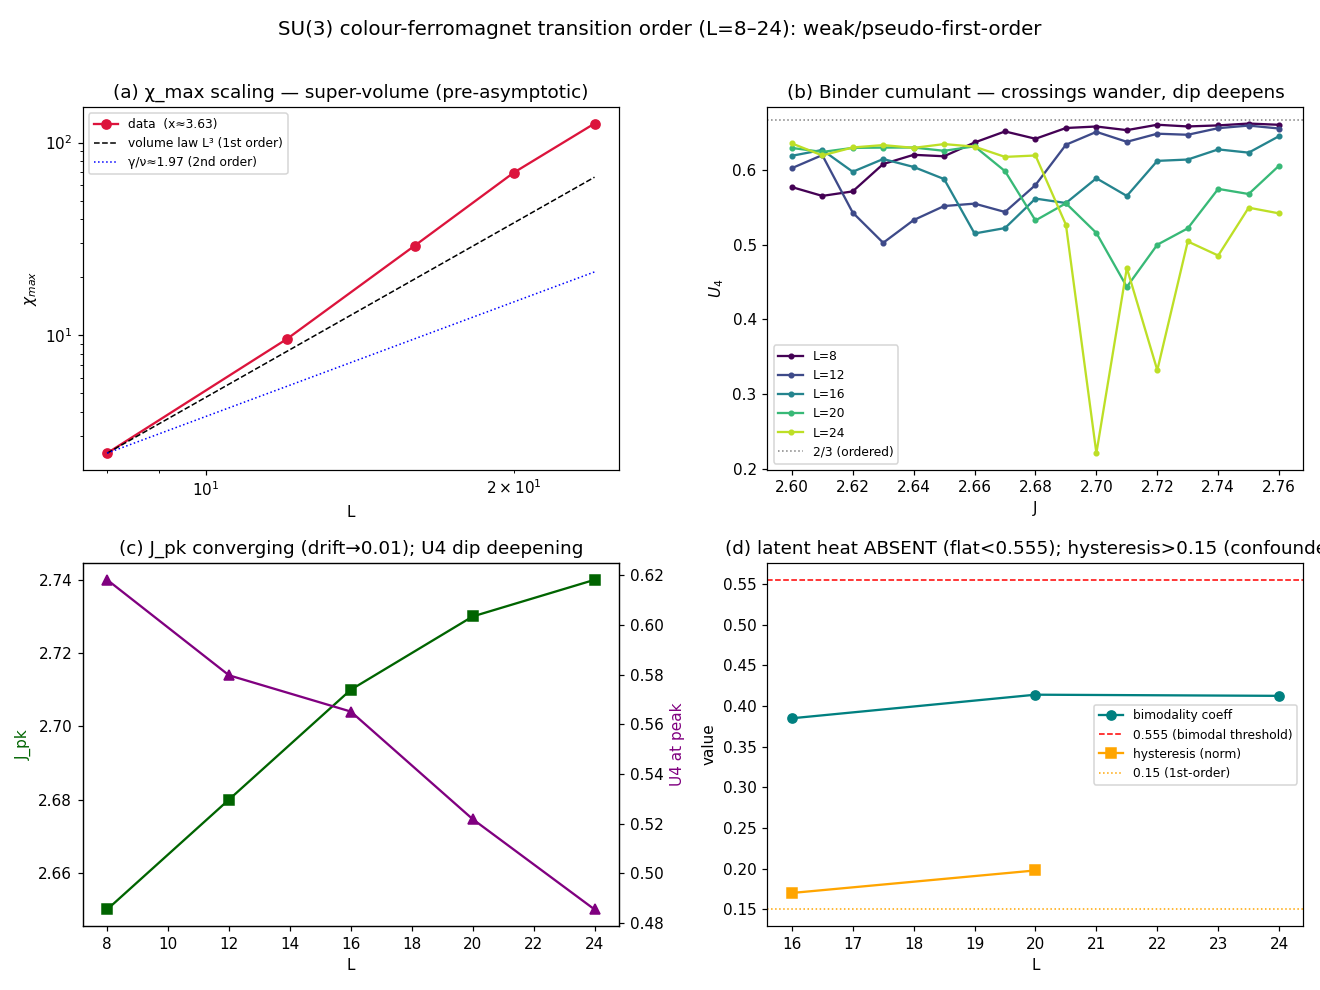
\includegraphics[width=\textwidth]{figures/su3/OT_order.png}
\caption{Order of the colour-ferromagnet transition, $L=8$--$24$. (a)~$\chi_{\max}$ grows
at least as the volume ($x_{\rm eff}\simeq3.6$, super-volume = pre-asymptotic), excluding a
clean second-order transition. (b)~Binder cumulant: the crossings wander and the dip
deepens with $L$. (c)~the susceptibility peak drifts upward and the $U_4$ dip deepens.
(d)~the latent heat (energy-histogram bimodality) is \emph{absent and flat} up to $L=24$,
bounding any first order to weak. Verdict: weak / pseudo-first-order, reinforced at $L=32$
by parallel tempering (bimodal histogram, sharp $\chi$ step, swap bottleneck at $J_c$); the
strong-versus-weak distinction needs $L\gtrsim48$ with multicanonical sampling on a cluster.}
\label{fig:order}
\end{figure*}

\section{Discussion}\label{sec:discussion}

\emph{Confinement and the octet are independent of the transition order.} The linear
potential, the positive string tension, the stable colour Skyrmion, and the exactly
degenerate octet are measured at fixed coupling deep in the ordered phase and follow from
the symmetry-breaking pattern and the area law; none depends on whether the ordering
transition is weakly first or continuous. The open question of \S\ref{sec:order} therefore
qualifies the \emph{description of the transition}, not the colour-sector results.

\emph{What is new relative to conventional lattice QCD.} The colour structure here is not
put in by hand as an $SU(3)$ gauge Lagrangian on a regular lattice; it is carried by an
internal field on a Lorentz-invariant Poisson causal order, and the ordering, the meson
octet, and confinement are emergent measurements on that substrate, sharing one vacuum with
the orientation/baryon sector of the companion papers \cite{GoldstonePRD,MatterGravityPRD}. The octet
degeneracy is proved exact (a single symmetry-forced stiffness) on both cubic and causal
graphs, rather than found approximately.

\emph{Absolute scales are external.} The substrate is dimensionless: $\rho_s$, $c$, the
Skyrmion charge, the octet degeneracy, and the dimensionless ratios are derived, but the
lattice-to-physical scale is not. The string tension $\sigma$, the Regge slope
$\alpha'=1/(2\pi\sigma)$ of the confining flux tube, and the meson scale ($m_\pi$, $f_\pi$
in GeV) are in lattice units and are not converted---the same external-scale frontier as
throughout the programme \cite{TEICDoc1}. The Skyrme stabiliser is likewise an external
input, required by the sign theorem Eq.~\eqref{eq:sign}, not a free choice. These are
stated, not hidden.

\emph{Next steps.} Resolving strong-versus-weak first order needs $L\gtrsim48$ with
multicanonical or cluster sampling to measure the free-energy barrier (interface tension)
directly---parallel tempering at $L=32$ reinforces the first-order reading but cannot cross
the barrier to weigh the two phases; the $SU(3)$ baryon sector (flavour collective
quantisation, richer than $SU(2)$)
and the coupling of the colour sector to the gravitational sector are the natural
continuations.

\section{Conclusion}\label{sec:conclusion}

On a single Poisson causal substrate, into which no chromodynamics was inserted, an $SU(3)$
internal field orders spontaneously into a colour ferromagnet (long-range order $C_\infty=m^2$
on the causal graph), supports a stable colour Skyrmion ($\pi_3(SU(3))=\mathbb{Z}$, $B=+1$) and
a confining linear potential (string tension $\sigma>0$, decreasing with the coupling), and
yields eight exactly degenerate Goldstone modes---the pseudoscalar meson octet, forced by the
unbroken $SU(3)_V$ adjoint with stiffness $\rho_s\simeq\tfrac13$ and speed $c=\sqrt{2/3}$. All
three are robust to a $\pm10\%$ deformation of the action. The ordering transition is not a
clean second-order transition---the susceptibility grows at least as the volume and the Binder
dip deepens---and is most probably weakly first order, reinforced at $L=32$ by parallel
tempering, though the latent heat stays unresolved (the tempering does not cross the barrier)
and the strong-versus-weak distinction awaits $L\gtrsim48$ multicanonical sampling. The contribution is a
structural, dimensionless one: colour order, confinement, and a meson octet emerge together
from a discrete causal substrate, with every absolute scale honestly external.

\begin{acknowledgments}
This work uses only the author's own simulations; the anti-circularity guard, the
implementation gates, and the pre-registered death criteria of the FL1, OS, FLR, and
SU3\_ORDEM campaigns are part of the build. Real QCD numbers are used only in labelled
comparison-only remarks, never as input.
\end{acknowledgments}

\bibliographystyle{apsrev4-2}
\bibliography{TEIC_CONSOLIDATED}

\end{document}
